\section{Windows Presentation Foundation}
Windows Presentation Foundation (WPF) er en grafisk brugergrænseflade på Windowsbaseret applikationer. 
WPF gør brug af  bl.a. vektorbaseret rendering af grafik, databinding, til nem redigering af data igennem den grafiske brugergrænseflade, og har også inkluderet Extensible Application Markup Language (XAML), hvilket er en nem måde at skabe WPF-grafik på.\citep{wpf} 

I dette projekt bruges WPF til at skabe den grafiske brugergrænseflade. Valget stod mellem WPF og Windows Forms (WinForms), hvilket er forgængeren til WPF til generering af grafik til Windows. 
Valget faldt på WPF, da XAML, som WinForms ikke har, gør det let at hurtigt lave en grafisk brugergrænseflade. 
Microsoft har også informeret om, at der ikke længere tilføjes nye funktioner til WinForms, men kun udelukkende rettelser af fejl.\citep{winforms}

En helt anden mulighed, som blev diskuteret, var at bruge en hjemmeside, som ville have den fordel, at den kan køre på stort set alle enheder, som har adgang til internettet via en browser. En hjemmeside, som gør brug af C\#, vil kunne laves lidt på samme måde som ved WPF; Med HTML (HyperText Markup Language) og CSS (Cascading Style Sheets) som frontend og C\#-klasser som backend. 
En hjemmeside blev fravalgt, da der blev vurderet at WPF var nemmere at oprette end en hjemmeside og at en grafisk brugergrænseflade ikke er det essentielle i opgaven. 

\subsection{Ofte anvendte WPF-controls}
Der anvendes ofte nogle få WPF-controls til at bygge brugergrænsefladen.
Disse vil blive beskrevet her.
På figur \ref{img:wpfdemo} vises de beskrevede elementer (Note de 3 sidste elementer er henholdsvis DataGrid, ComboBox og ListBox).


\subsubsection{ComboBox}
I WPF er en ComboBox det element som andre steder omtales som en dropdown menu. 
Dens indhold kan instilles enten i XAML-koden eller i Code-Behind koden.
Hvis dette indhold skal være dynamisk, vil Code-Behind ofte være anvendt.
Eksempelvis hvis man kun vil have de medlemmer af en liste som opfylder et givent prædikat. 

\subsubsection{Button}
En Button er en knap, knappen kalder en methode i Code-Behind koden. 
Den metode udfører et stykke arbejde.

\subsubsection{DataGrid}
Et DataGrid er et grafisk element som kan vise data dynamisk.
Ofte vil det vise en liste af objekter af en klasse.
Dets layout er opdelt i rækker og kolloner, hvor hver kollone indeholder en bestemt type data, og kan sorteres ved at klikke på labellet.
Det er også muligt at konstruere en søgefunktion, altså kan et DataGrid bliver filteret.

\begin{wrapfigure}[22]{R}{0.5\textwidth}
    \label{img:wpfdemo}
    \vspace{-30pt}
    \begin{center}
        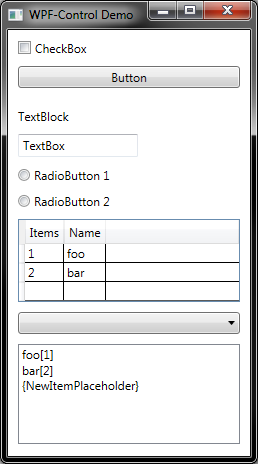
\includegraphics[width=0.48\textwidth]{UI/WPF-Demo.png}
    \end{center}
    \vspace{-15pt}
    \caption{Demonstration af WPFs Controls}
\end{wrapfigure}

\subsubsection{CheckBox}
En CheckBox er en kvadratisk boks, som enten er ``Checked'' eller ikke ``Checked''. 
Dens stadie et binært, og (som standard) uafhængig af andre elementer.

\subsubsection{RadioButton}
En RadioButton er en cirkelformet CheckBox.
Dog vil RadioButtons ofte optræde i serie, altså 2 eller flere sammen.
Et oplagt brug af dem er til ja, nej (og måske), situationer, hvor kun en af dem skal vælges.

\subsubsection{StackPanel}
Et stackpanel er ikke synligt for slutbrugeren, men bruges til at organisere de andre grafiske elementer.
Pricippet er at alle elementer i et StackPanel, bliver skubbet sammen i mod en given retning.
Dette gør det nemmere at få de grafiske elementer til at flugte.
Derudover sikrer det en konsistet bredde af elementer deri, med mindre andet angivet.

\subsubsection{TextBlock}
En TextBlock er det stykke læs-kun tekst.
Det vil typisk være en forklarende tekst, op ad et andet grafisk element.
Det er også muligt at ændre en TextBlock via Code-Behind. 
Hvis man vil føre en dialog med brugeren, eksempelvis til fejlbeskeder.

\subsubsection{TextBox}
En TextBox er et tekstfelt, hvori brugeren kan skrive infomation. 
Dette kan dermed ses som et inputfelt. 
Det er også muligt at sætte sådan et felt til at være skrivebeskyttet, samt at ændre dets indhold.

\subsubsection{ListBox}
En ListBox er en tabel, med en kollone og flere rækker, hvori en bruger kan vælge en eller flere elementer.
ListBoxen er i stand til at indeholde samlinger af data på enhverform, oftest vil det være en streng, men et billede er også en mulighed.
Den vil i nogen tilfælde have samme brugsscenarie som en ComboBox eller et DataGrid. 
Forskellen fra en ComboBox er at der kan være flere synlige elementer, i en ListBox på samme tid, samt der ikke er nogen dropdown menu.
Et DataGrid kan indeholde flere infomationer, på kolloner, mens en ListBox kun kan indeholde en infomation.

\subsubsection{UserControls}
Det er mulig at konstruere sine egne grænseflade elementer, fra et ellere flere at WPFs indbyggede eller 3. parts Controls.
Dette kaldes en UserControl, denne indholder både en grafisk del og en Code-Behind.
Det brugerskabte element, kan derefter genbruges flere stedder i programmet.
Dette er et eksempel på genanvendelse, hvilket kan bidrage til højere program kvalitet, og større konsistens gennem programmet. 

